\documentclass[a4paper, 12pt]{article}
\usepackage[usenames,dvipsnames,svgnames,table]{xcolor}
\usepackage[T1]{fontenc}
\usepackage{times}
\usepackage{multirow}
\usepackage{float}
\usepackage{amssymb}% http://ctan.org/pkg/amssymb
\usepackage{pifont}% http://ctan.org/pkg/pifont
\usepackage[utf8]{inputenc}
\usepackage{wallpaper}
\usepackage[absolute]{textpos}
\usepackage[top=2cm, bottom=2.5cm, left=3cm, right=3cm]{geometry}

\newsavebox{\mybox}
\newlength{\mydepth}
\newlength{\myheight}
\newenvironment{sidebar}
{\begin{lrbox}{\mybox}\begin{minipage}{\textwidth}}
{\end{minipage}\end{lrbox}
 \settodepth{\mydepth}{\usebox{\mybox}}
 \settoheight{\myheight}{\usebox{\mybox}}
 \addtolength{\myheight}{\mydepth}
 \noindent\makebox[0pt]{\hspace{-20pt}\rule[-\mydepth]{1pt}{\myheight}}
 \usebox{\mybox}}

\newcommand{\cmark}{\ding{51}}%
\newcommand{\xmark}{\ding{55}}%

\newcommand\BackgroundPic{
    \put(-2,-3){
    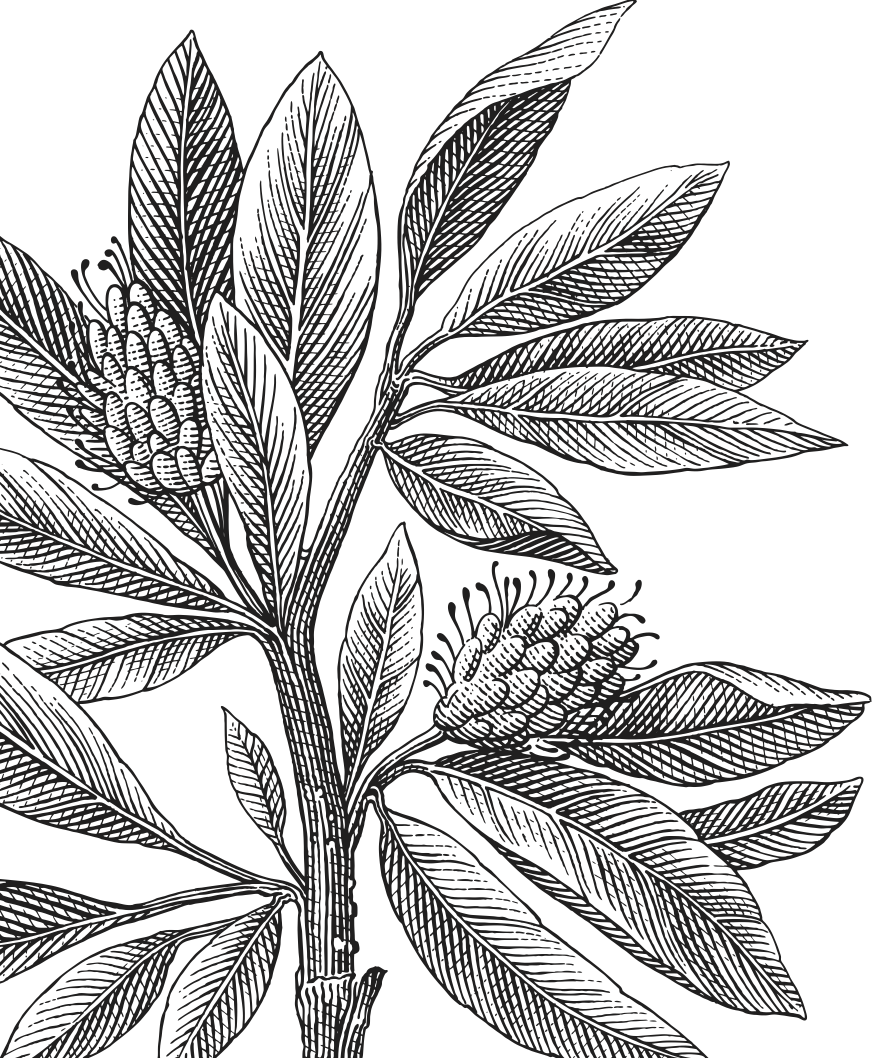
\includegraphics[keepaspectratio,scale=0.3]{../lnu_etch.png} 
    }
}
\newcommand\BackgroundPicLogo{
    \put(30,740){
	
\includegraphics[keepaspectratio,scale=0.10]{../logo.png}     
    }
}

\title{	
\vspace{-8cm}
\begin{sidebar}
    \vspace{5cm}
    \normalfont \normalsize
    \Huge Report \\
    \vspace{-1.3cm}
\end{sidebar}
\vspace{3cm}
\begin{flushleft}
    \huge Test Report\\  
\end{flushleft}
\null
\vfill
\begin{textblock}{6}(10,13)
\begin{flushright}
\begin{minipage}{\textwidth}
\begin{flushleft} \large
	\emph{Author:} Anonymous \\
	%\emph{Handledare:} \\ 
	\emph{Term:} HT 2017\\ 
	\emph{Course:} 2DV610 - Software Testing\\
\end{flushleft}
\end{minipage}
\end{flushright}
\end{textblock}
}
\date{\today} 

\begin{document}

\pagenumbering{gobble}
\newgeometry{left=5cm}
\AddToShipoutPicture*{\BackgroundPic}
\AddToShipoutPicture*{\BackgroundPicLogo}
\maketitle
\restoregeometry
\clearpage

\pagenumbering{gobble}

\tableofcontents
\newpage
\pagenumbering{arabic}

\section{Licence Compatibility}
\textbf{Requirement 4: The server should be released under GPL-2.0} \\
MyWebServer has previously been released under MIT which is compatible with GPL-2.0 and it should not cause any complications \footnote{https://www.gnu.org/licenses/license-list.en.html\#Expat}. However, to avoid release complications the server should be distributed with \textit{OpenJDK} which is licensed under GPL-2.0 \footnote{http://openjdk.java.net/legal/gplv2+ce.html}. The server executable should also be striped of \textit{JUnit 4.12} which is licensed under ELC and is therefore not compatible with GPL-2.0 \footnote{http://junit.org/junit4/license.html} \footnote{https://www.gnu.org/licenses/license-list.en.html\#EPL}. It would also be preferred to remove \textit{Mockito} from the executable even if it's released under MIT which is compatible with GPL-2.0. 


\section{Traceability Matrix}

\begin{tabular}{|c|c|c|c|c|c|c|c|c|}
\hline
\multicolumn{8}{|c|}{Requirement Matrix} \\ \hline
Requirement	& Reqs		& Req. 1	& 	Req. 2	&  Req. 3	& Req. 5 	& Informal	& Informal	\\ 
Identifiers		& Tested	&				&				& 				&				&	Req. 1	&	Req. 2	\\ \hline
Test Cases	&	38			&	1			&	4			&	16			&	3			&	10			&	4			\\ \hline
1.1				& 	2			&				&				&	X			&				&	X			&				\\ \hline
1.2				& 	3			&				&				&	X			&				&	X			& X			\\ \hline
1.3 				& 	3			&				&				&	X			& X			&	X			&				\\ \hline
1.4				&	2			&				&				&  X			&				&	X			&				\\ \hline
2.1				&	2			& 				& 				&	X			&				&	X			&				\\ \hline
2.2				&	3			&				& 				&	X			& X			&	X			&				\\ \hline
3.1				&	2			&				& X			&	X			&				&				&				\\ \hline
3.2				&	2			&				& X			&	X			&				&				&				\\ \hline
3.3				&	2			&				& X			&	X			&				&				&				\\ \hline
3.4				&	2			&				& X			&	X			&				&				&				\\ \hline
4.1				& 	4			&	X			& 				&	X			& 				& X			& X			\\ \hline
5.1				&	3			&				&				&	X			& X			& X			&				\\ \hline
6.1				&	2			&				&				&	X			&				& X			&				\\ \hline
6.2				&	2			&				&				&	X			&				& X			&				\\ \hline
7.1				&	2			&				&				&	X			&				&				& X			\\ \hline
7.2				&	2			&				&				&  X			&				&				& X			\\ \hline

\end{tabular}

\newpage
\section{Test Cases - Result}

\textit{\cmark = Pass, \xmark = Fail} \\

\begin{tabular}{| c | l | l | l | l | c |}
\hline

Test Case 		& OS		& Expected Output		& Actual Output		& Date		& Pass		\\ \hline
\multirow{2}{*}{1.1}    & Mac		& Unable to connect		& As expected		& 21/12	        &\cmark		\\ 
			&		& Socket 80 was taken		& Port is taken		& 21/12		&\xmark		\\ 
\cline{2-6}		& Linux		& Unable to connect		& As expected		& 21/12		& \cmark	\\
			&		& Socket 80 was taken		& Port is taken		& 21/12		& \xmark	\\ \hline
\multirow{2}{*}{1.2}	& Mac		& No access to folder		& HTTP Server 		& 21/12		& \xmark	\\ 
			&		& /var/root/			& Started		&		&		\\
\cline{2-6}		& Linux		& No access too folder		& HTTP Server 		& 21/12		& \xmark	\\ 
			&		& /root/			& Started		&		&		\\ \hline
\multirow{2}{*}{1.3}	& Mac		& Cannot write to server	& HTTP Server 		& 21/12		& \xmark	\\ 
			&		& log file log.txt		& Started		&		&		\\
\cline{2-6}		& Linux		& Cannot write to server	& HTTP Server		& 21/12		& \xmark	\\ 
			&		& log file log.txt		& Started		&		&		\\ \hline
\multirow{2}{*}{1.4}	& Mac		& HTTP Server Started		& As expected		& 21/12		& \cmark 	\\ 
			&		& It Works			& As expected		& 21/12		& \cmark 	\\
\cline{2-6}		& Linux		& HTTP Server Started		& As expected		& 21/12		& \cmark	\\ 
			&		& It Works			& As expected		& 21/12		& \cmark 	\\ \hline
\multirow{2}{*}{2.1}	& Mac		& Unable to connect		& As expected		& 21/12		& \cmark	\\
\cline{2-6}		& Linux		& Unable to connect		& As expected		& 21/12		& \cmark	\\ \hline
\multirow{2}{*}{2.2}	& Mac		& HTTP Server stopped		& Only written in	& 21/12		& \xmark	\\
			&		& written in access log		& console		& 		& 		\\
\cline{2-6}		& Linux		& HTTP Server stopped		& Only written in	& 21/12		& \xmark	\\ 
			&		& written in access log		& console		& 		& 		\\ \hline
\multirow{2}{*}{3.1}	& Mac		& Response Code 200		& As expected 		& 21/12		& \cmark	\\
\cline{2-6}		& Linux		& Response Code 200		& As expected 		& 21/12		& \cmark	\\ \hline
\multirow{2}{*}{3.2}	& Mac		& Response Code 404 		& As expected 		& 21/12		& \cmark	\\
\cline{2-6}		& Linux		& Response Code 404		& As expected 		& 21/12		& \cmark	\\ \hline
\multirow{2}{*}{3.3}	& Mac		& Response Code 403		& As expected 		& 21/12		& \cmark	\\
\cline{2-6}		& Linux		& Response Code 403		& As expected 		& 21/12		& \cmark	\\ \hline
\multirow{2}{*}{3.4}	& Mac		& Response Code 400		& As expected 		& 21/12		& \cmark	\\
\cline{2-6}		& Linux		& Response Code 400		& As expected 		& 21/12		& \cmark	\\ \hline
\multirow{2}{*}{4.1}	& Mac		& Response time <2000		& 127 ms		& 21/12		& \cmark	\\
\cline{2-6}		& Linux		& Response time <2000		& 87 ms			& 21/12		& \cmark	\\ \hline
\multirow{2}{*}{5.1}	& Mac		& Clientthread <nr>		& Only written in	& 21/12		& \xmark	\\
			&		& served file : works.png 	& console		&		&		\\
\cline{2-6}		& Linux		& Clientthread <nr>		& Only written in	& 21/12		& \xmark	\\
			&		& served file : works.png 	& console		&		&		\\ \hline
\end{tabular}

\newpage

\begin{tabular}{| c | l | l | l | l | c |}
\hline

Test Case 		& OS		& Expected Output		& Actual Output		& Date		& Pass		\\ \hline
\multirow{2}{*}{6.1}	& Mac		& Enter a valid port		& As expected		& 21/12		& \cmark	\\
			&		& 1-65 535 and a 		&			&		&		\\
			&		& optional URL			&			&		&		\\
\cline{2-6}		& Linux		& Enter a valid port		& As expected		& 21/12		& \cmark	\\
			&		& 1-65 535 and a 		&			&		&		\\
			&		& optional URL			&			&		&		\\ \hline
\multirow{2}{*}{6.2}	& Mac		& \textit{See fig. \ref{HSc}}	& Enter a valid port	& 21/12		& \xmark	\\
			&		&				& 1-65 535 and a	&		&		\\
			&		&				& optional URL		&		&		\\
\cline{2-6}		& Linux		& \textit{See fig. \ref{HSc}}	& Enter a valid port	& 21/12		& \xmark	\\ 	
			&		&				& 1-65 535 and a	&		&		\\
			&		&				& optional URL		&		&		\\ \hline
\multirow{2}{*}{7.1}	& Mac		& It Works			& Safari could not	& 21/12		& \xmark	\\
			&		&				& open page		&		&		\\
\cline{2-6}		& Linux		& It Works			& Secure connection	& 21/12		& \xmark	\\ 
			&		&				& failed		&		&		\\ \hline
\multirow{2}{*}{7.2}	& Mac		& Response Code 405		& As expected		& 21/12		& \cmark	\\
\cline{2-6}		& Linux		& Response Code 405		& As expected		& 21/12		& \cmark	\\ \hline	
\end{tabular}

\begin{figure}[H]
\centering
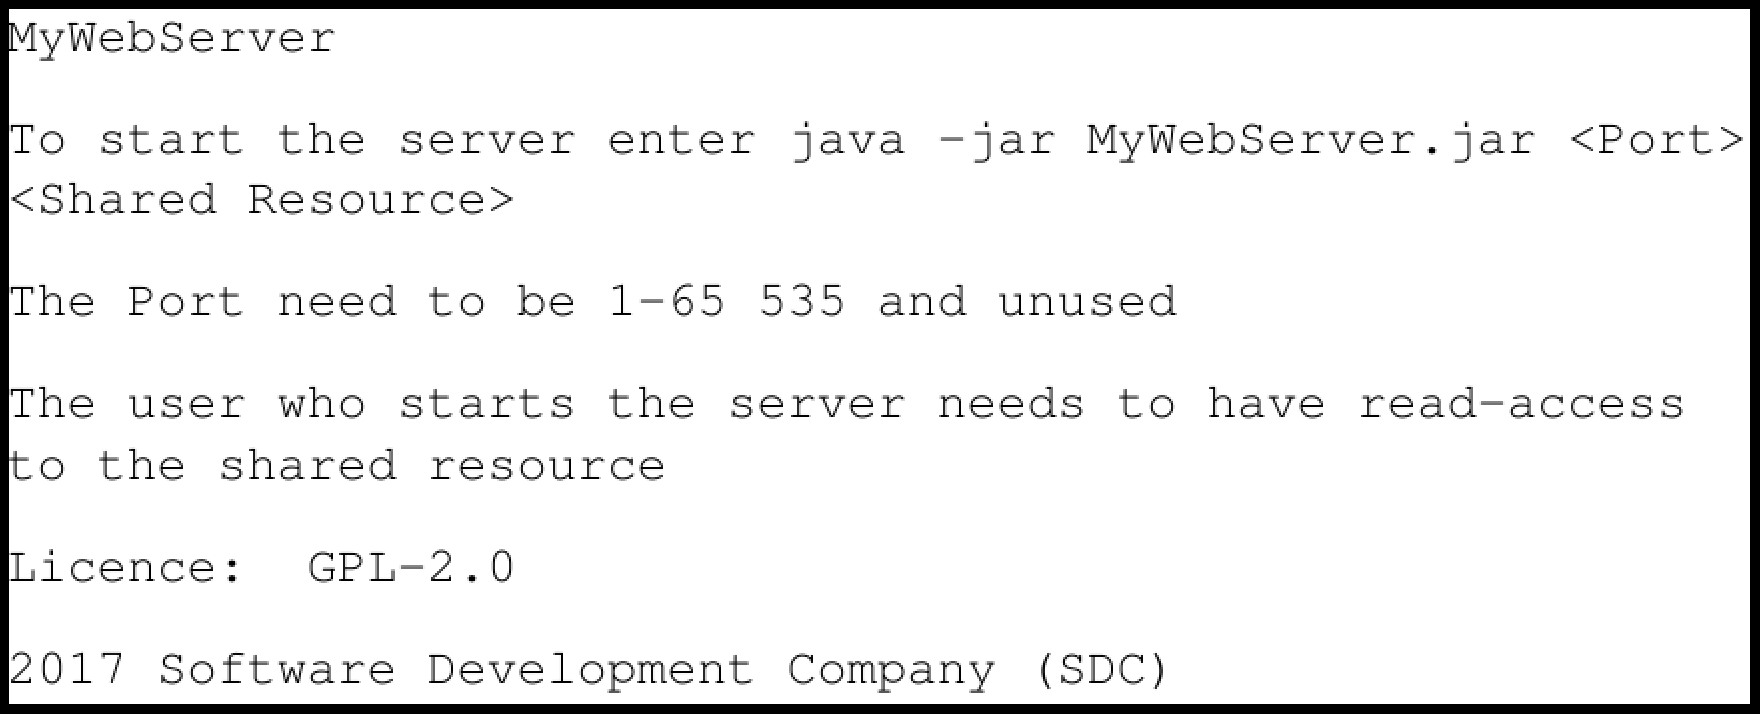
\includegraphics[scale=0.5]{help_screen.png}
\caption{Help screen}
\label{HSc}
\end{figure}
\newpage

\end{document}
